\documentclass{article}
\usepackage[utf8]{inputenc}
\usepackage{amsmath}
\usepackage{amssymb}
\usepackage{graphicx}
\usepackage[dvipsnames]{xcolor}
\usepackage{float}


\newcommand{\indep}{\perp\!\!\!\!\perp} 

\title{Causal Mediation Analysis}
\author{Julian Ashwin}
\date{August 2022}

\begin{document}
	
	\maketitle
	
	\section{Introduction}
	
	
	Basic set up:
	\begin{itemize}
		\item $T_i$ is treatment status for $i$
		\item $M_i(t)$ is the potential value of a mediator for $i$ under treatment $T_i = t$
		\item $Y_i(t,m)$ is potential outcome from treatment $t$ and mediator $m$. 
	\end{itemize}
	Total treatment effect is therefore
	$$
	\tau_i \equiv Y_i(1, M_i(1)) - Y_i(0,M_i(0)).
	$$
	This total treatment effect is made up of two components, a causal mediation effect:
	$$
	\delta_i(t) \equiv Y_i(t, M_i(1)) - Y_i(t,M_i(0)).
	$$
	All other mechanisms are represented as the direct effects of the treatment
	$$
	\zeta_i(t) \equiv
	$$
	The average causal mediation effect (ACME) is $\bar{\delta}(t)$ and the average direct effect (ADE) is $\bar{\zeta}(t)$. 
	\\~\\
	Identification of the ACME requires an assumption of sequential ignorability. 
	\begin{equation}
		\{Y_i(t',m), M_i(t)\} \indep T_i | X_i = x 
	\end{equation}
	which is the standard strong ignorability of the treatment assignment (i.e. conditional on $x$ treatment is effectively randomly assigned). 
	\begin{equation}
		Y_i(t',m) \indep , M_i(t) | T_i =t, X_i = x 
	\end{equation}
	which requires that the mediator is also ignorable given treatment and confounders. This is quite strong as it rules out the possibility of multiple mediators that are related to one another. Later on we will show results if there are multiple mediators. 
	
	
	\section{Model-based CMA}
	
	Two steps:
	\begin{enumerate}
		\item Specify two statistical models: mediator model for the conditional distribution of $M$ given $T$ and $X$; and the outcome model for the conditional distribution of $Y$ given $T$, $M$ and $X$. These models are estimated separately.
		\item Compute the ACME and other quantities of interest from the mediator and outcome models. 
	\end{enumerate}
	Since the sequential ignorability assumption is untestable, we can conduct a sensitivity analysis. 
	\\~\\
	mediate function takes model objects corresponing to the mediator and outcome models and calculates the ACME following the algorithm described in Imai et al (2010a). These algorithms overcome the limitation of the standard methods based on the product or difference of coefficients, which only work if both mediator and outcome models are linear regressions where $T$ and $M$ enter additively.
	\\~\\
	\textbf{Treatment and mediator interaction.} It could be that the ACME takes different values depending on the baseline treatment status. For this just include and interaction between treatment and mediator in the outcome model. We then get and ACME that varies with the treatment status.
	
	\subsection{Moderated mediation}
	
	The magnitude of the ACME may depends on a pre-treatment covariate (called the moderator). There are two alternative routes to analyse moderated mediation with the package.
	\begin{enumerate}
		\item Include the moderator and interactions in the outcome and mediator models, interacted with both $T$ and $M$. Then specify the levels of the moderator at which to calculate the ACME using the covariates argument. 
		\item Test the significance of the difference between ACME and ADE between two chosen levels of covariate using the test.modmed function. 
	\end{enumerate}
	
	
	\subsection{Sensitivity analysis for sequential ignorability}
	
	For example, choose as the sensitivity parameter the correlation $\rho$ between residuals of the mediator and outcome regressions. If there are pre-treatment confounders which affect both the mediator and the outcome, the sequential ignorability assumption is violated and $\rho \neq 0$. The sensitivity analysis is conducted by varying the value of $\rho$ and examining how the ACME changes. 
	\\~\\
	In the vignette example, the confidence interval for the ACME contains zero for $\rho = 0.3$ and $\rho = 0.4$. 
	\\~\\
	This sensitivity analysis seems to capture how the results change if we introduce extra confounders or something? Rather than a test of the sequential ignorability function itself. 
	\\~\\ 
	I skipped the Section on multilevel data for now. 
	\\~\\
	There is a Section on design-based causal mediation analysis, which is a more fully non-parametric approach. 
	
	\section{Causally dependent multiple mechanisms}
	
	Accounting for alternative mechanisms often crucial for the identification of the mechanism of primary interest. 
	\\~\\
	Imai and Yamamoto (2013) develop methods for dealing with multiple mediators. 
	\begin{itemize}
		\item When the mediators are not causally related, this is not that difficult. For each mediator, the other mediators are neither pre-treatment nor post-treatment confounders. The effects can thus be consistently estimated by applying the mediate function successively to each one, ignoring the existence of other mediators.
		\item When multiple mediators are causally related (or equivalently when one mediator acts as a post-treatment confounder for the other) the analysis requires new assumptions. 
	\end{itemize}
	~\\
	Let $W_i(t)$ be the vector of potential values of alternative mediators given treatment status $t$. Allow the causal dependence of the primary mediator $M_i(t,w)$ and the outcome $Y_i(t,m,w)$ on $W$. The causal mediation effect is then expressed as 
	$$
	\delta_i(t) = Y_i(t, M_i(1, W_i(1)), W_i(t) - Y_i(t, M_i(0, W_i(0), W_i(t))
	$$
	Noting that this is the effect transmitted through the primary mediator $M_i$, irrespective of $W_i$. 
	\\~\\
	In Imai and Yamamoto (2013), analysis is based on varying coefficient linear SEM
	$$
	M_i(t,w) = \alpha_2 + \beta_{2,i}t + \zeta_{2,i} w + \mu_{2,i} t w + \lambda_{2,i} x + \epsilon_{2,i}
	$$
	$$
	Y_i(t,m,w) = \alpha_3 + \beta_{3,i}t + \gamma_i m + \kappa_i t m + \zeta_{3,i} w + \mu_{3,i}tw + \lambda_{3,i} x + \epsilon_{3,i}
	$$
	were these are super flexible as the coefficients can vary across individual units. There are two strategies for analysing the average causal mediation effect $\bar{\delta}(t)$.
	\begin{enumerate}
		\item Show that the ACME is point identified under the above model and sequential ignorability if homogeneous interaction is satisfied:
		$$
		Y_i(1,m,W_i(1)) - Y_i(0,m,W_i(0)) = B_i + Cm
		$$
		This states that the degree of interaction between treatment and primary mediator $m$ is constant across individuals.
		\item When this assumption is violated, we can express bounds on the ACME as functions of a parameter representing the degree of violation and conduct a sensitivity analysis wrt the deviation of the coefficient on the treatment mediator interaction term: $\sigma \equiv \sqrt{Var(\kappa_i)}$.
	\end{enumerate}
	
	The SEM framework is implemented as the multimed function. This takes a data frame containing the necessary variables (outcome, primary mediator, alternative mediator, treatment, and pre-treatment covariates). This function has pretty different arguments:
	\begin{itemize}
		\item name of outcome 
		\item first mediator
		\item second mediator
		\item treatment
		\item pre-treatment covariates to condition on
	\end{itemize}
	As an example, use continuous outcome (immigr). Main mediator is the composite measure of anxiety (emo), the treatment (treat) is exposure to media stories, and the pre-treatment covariates are age, education, gender and income. The alternative mediator is p\_harm, which is a measure of perceived economic harm. 
	\\~\\
	This produces two tables showing the estimated effects and some sensitivity results. 
	
	
	
	\section{Notes on Imai et al (2011)}
	
	Traditional approach to causal mediation is through structural equation models. This relies on untestable assumptions and these are often insufficient - conventional exogeneity assumptions are insufficient for identification of causal mechanisms. This paper makes three contributions:
	\begin{enumerate}
		\item Minimum set of assumptions under experimental and observational studies, showing that conventional exogeneity assumptions are insufficient. Then develop a general alogirthm for estimating causal mediation effects, correcting common mistakes. 
		\item Sensitivity analysis to violations of key assumptions. 
		\item Provide alternative research designs to enable identification of causal mechanisms under less stringent assumptions. 
	\end{enumerate}
	Illustrate with two empirical examples: media priming and observational studies of incumbency advantage. 
	\\~\\
	\textbf{Decomposing incumbency effects.} Incumbency advantage is one of the most studied topics in electoral politics. Many potential mechanisms like "scare-off/quality effect" - deterring high quality challengers, name recognition and resource advantage. 
	\\~\\
	\textbf{Potential Outcomes refresher.} With binary treatment, there are two potential outcomes until one is realised and the other remains unobserved. So $Y_i(t)$ is the potential outcome for unit $i$ under the treatment status $t$. 
	\\~\\
	In observational studied, treatments are not randomised, so we often adjust for the observed differences in the pretreatment covariates $X_i$ between the treatment and control groups through regression, matching etc... This assumes that there are no omitted variables that affect both treatment and outcome, so $\{Y_i(1), Y_i(0)\} \indep T_i | X_i = x$. For example, controlling for lagged values of the dependent variable.
	\\~\\
	Under this framework, the ATE is the average difference in outcome means between treatment and control groups. 
	\\~\\
	\textbf{Defining Causal Mechanisms as Indirect and Direct Effects.} In the Cox and Katz case, challenger quality is the mediator (M) through which the incumbency status (T) causally affects the election outcome (Y). As there are other potential mechanisms, an inferential goal is to decompose the causal effect into indirect (the mediator) and direct (all other mechanisms). The total treatment effect is
	$$
	\tau_i \equiv Y_i(1, M_i(1)) - Y_i(0,M_i(0))
	$$
	The indirect/causal mediation effect us
	$$
	\delta_i(t) \equiv Y_i(t,M_i(1)) - Y_i(t, M_i(0))
	$$
	This represents the indirect effects of the treatment on the outcome through the mediating variable. By fixing the treatment and changing only the mediator we eliminate all other causal mechanisms and isolate the hypothesized mechanism. In the Cox and Katz (1996) study, then the indirect effect $\delta_i(1)$ is the difference between the observed vote share $Y_i(1,M_i(1))$ and the counterfactual vote share $Y_i(1, M_i(0))$, i.e.e the vote share if the candidate would receive if he or she faced a challenger whose quality was at the same level as the challenger he or she would have faced if not an incumbent. This thus isolates the portion of the incumbency advantage due to the quality effect. 
	\\~\\
	All other causal mechanisms are then the direct effects of the treatment 
	$$
	\zeta_i(t) \equiv Y_i(1, M_i(t)) - Y_i(0,M_i(t))
	$$
	In the incumbency example, $\zeta_i(t)$ represents the difference in vote share of candidate $i$ with and without incumbency status holding the challenger quality at the level that would be realised if the candidate was an incumbent. 
	\\~\\
	Goal is to decompose the ATE into the ACME and the ADE and assess the relative important of the hypothesized mechanism. 
	
	\subsection{Nonparameteric Identification under Standard Designs}
	
	Standard design - treatment assignment is either randomized or assumed to be random given the pre-treatment covariates. Identifying the causal mechanism requires an additional assumption: the Sequential Ignorability assumption. 
	\begin{equation}
		\{Y_i(t',m), M_i(t)\} \indep T_i | X_i = x 
	\end{equation}
	\begin{equation}
		Y_i(t',m) \indep , M_i(t) | T_i =t, X_i = x 
	\end{equation}
	First, given observed pre-treatment confounders, the treatment assignment is assumed to be ignorable (i.e. statistically independent of potential outcomes and potential mediators) - this is the standard no-omitted-variable bias, exogeneity or unconfoundedness assumption. 
	\\~\\
	Second, we assume that the observed mediator is ignorable given the actual treatment status and pre-treatment confounders. In other words, once we have conditioned on a set of covariates, the mediator status is ignorable. This is similar to the standard assumption that treatment assignment is exogenous in observational studies - so even if treatment is truly randomised then this assumption is still reasonably strong. 
	\\~\\
	In the incumbency advantage example, the first part needs to be considered carefully as the treatment is not randomised - we need to assume that incumbency status is random once we adjust for differences in the previous election outcome and partisanship. Furthermore, we also require that the quality of the challenger in the current election is random once we take into account differences in the incumbency status and past election outcomes and partisanship. For both these cases, there may exist unobserved confounders. It is generally impossible to entirely rule out the possibility that there are some unobserved variables which confound relationships, even after conditioning on observable covariates. 
	\\~\\
	However, if we make these assumptions, then both the ACME and the ADE are nonparametrically identified, so can be identified without any additional distributional or functional form assumptions. 
	\\~\\
	Note that even if both treatment and mediator are randomly assigned, sequential ignorability does not necessarily hold. This is because there is a fundamental difference between the causal effect of the mediator itself and the causal mediation effect. The causal mechanism represents how the effect of \textit{treatment} on outcome is transmitted through the mediator. Identifying the effect of the mediator itself is not sufficient to identify the causal mediation effect. 
	\\~\\
	The sequential ignorability assumption requires that the covariates conditioned on only include \textit{pre-treatment} variables (post-treatment confounders require additional strong assumptions for the ACME to be identified, such as no interaction between the treatment and mediator, Robins (2003)). We cannot condition on premediator confounders if they are affected by the treatment. 
	\\~\\
	If the two causal mediators are unrelated, then the ACME for each mediator can be identified as before. In contrast, if there is a causal relationship between one mediator ($M$) and another mediator ($N$), then sequential ignorability is not satisfied even if both treatments are exogenous. 
	\\~\\
	For example, if the media cue effect goes through both emotion and cognitive mechanisms but these are entirely unrelated, then sequential ignorability holds. However, if beliefs about economic costs then go on to affect anxiety, then sequential ignorability does not hold. 
	\\~\\
	\textbf{Inference and sensitivity analysis under standard designs.} Approach here is not tied to any specific statistical model - parametric or non-parametric regressions can be used to model the mediator and outcome variables as the identification assumption does not specify a model. There is also a sensitivity analysis to probe the sequential ignorability assumption by quantifying the degree of possible violation. 
	\\~\\
	Standard approach to estimating mediation effects is to use linear equations. The effect of $T$ on $Y$
	$$
	Y_i = \alpha_1 + \beta_1 T_i + \xi_1 X_i + \epsilon_{i1}
	$$
	The effect of $T$ on $M$
	$$
	M_i = \alpha_2 + \beta_2 T_i + \xi_2 X_i + \epsilon_{i2}
	$$
	The effect of $T$ and $M$ on $Y$
	$$
	Y_i = \alpha_3 + \beta_3 T_i + \gamma M_i + \xi_3 X_i + \epsilon_{i3}
	$$
	The standard method is to estimate ACME using the product of $\beta_2 \gamma$, or alternatively the difference $\beta_1 - \beta_3$. Sequential ignorability here implies zero correlation between $\epsilon_{i2}$ and $\epsilon_{i3}$. 
	\\~\\
	\textbf{Estimation Method.} As long as sequential ignorability holds, any statistical model can be used to compute the ACME and ADE. The algorithm has two steps:
	\begin{enumerate}
		\item Fit regression models for mediator and outcome. The mediator is modeled as a function of the treatment and any relevant pre-treatment covariate. This gives two sets of predictions for the mediator - with and without the treatment. 
		\item Use the outcome model to make potential outcome predictions. If we are interested in the ACME under treatment, predict outcome under treatment using value of mediator predicted in treatment condition, then the outcome under the treatment condition but with the mediator prediction from the control condition. The ACME is then the difference between the outcome predictions using the two different values of the mediator. So this corresponds to the average difference in volatility from fixing treatment status but changing volume between levels with and without a FT article.
	\end{enumerate}
	Uncertainty can then be computed with bootstraps or Monte Carlo approximations. 
	\\~\\
	\textbf{Sensitivity analysis.} Identifying the causal mechanism requires sequential ignorability, which cannot be tested with the observed data. But we can evaluate the robustness of empirical results to a violation of this assumption. This tests whether a slight violation of the assumption of sequential ignorability would lead to substantively different conclusions. 
	\\~\\
	Following Imai, Keele and Tingley (2010) and Imai, Keele and Yamamoto (2010), define $\rho$ as the correlation between $\epsilon_{i2}$, the error in the mediation model, and $\epsilon_{i3}$, the error in the outcome model. If sequential ignorability holds, all relevant pre-treatment confounders have been conditioned on and so $\rho$ is equal to zero. However, if $\rho$ is non zero then some hidden confounder is biasing the ACME estimate. In other words, there is some factor which both affects the outcome and the mediator in some way. This could for example be if there is genuinely new information contained in the news articles. This could both affect volatility and trading volumes that day. Although $\rho$ is unknown, we can calculate the values of $\rho$ for which the ACME is zero/not significant. 
	\\~\\
	This illustrates how even if the exogeneity assumptions hold for both $T$ and $M$, we can still get a biased estimate of the ACME if the outcome is not independent of the mediator conditional on treatment and covariates. 
	\\~\\
	The interpretation of $\rho$ is perhaps a little obscure, so instead Imai, Keele and Yamamoto (2010) provide an alternative formulation based on how much the omitted variable would alter the $R^2$ of the mediator and outcome models. For example, if information in the news articles is important in determining volatility or trading volume, then the model excluding this information will have a much smaller $R^2$ than the model that includes it. The relative change in $R^2$ can be used as a sensitivity parameter - e.g. if the confounding factor would only need to explain a very small portion of the remaining variance for the effect to lose significance, then the effect would be quite weak. 
	\\~\\
	This sensitivity analysis of course has limitations:
	\begin{enumerate}
		\item It is designed to mimic a pre-treatment confounder, so does not address confounders that are affected by the treatment and confound the relationship between the mediator and the outcome. Imai and Yamamoto (2011) do consider the case of post-treatment confounders though. 
		\item Sensitivity analysis does not provide any objective criterion to assess sequential ignorability, as it is an irrefutable assumption, so the best it can do is provide some suggestive evidence. 
	\end{enumerate}
	~\\
	
	
	
	\subsection{Applications}
	
	\textbf{The Media Framing experiment.} The research question here is how and why media cues influence attitudes towards immigration. Two possible factors:
	\begin{enumerate}
		\item Emphasising cost to society should increase opposition (and vice versa for benefits). 
		\item Whites more likely to oppose immigration when immigrants are non-white. 
	\end{enumerate}
	Two possible channels - cues operate through anxiety or through changing beliefs about costs and benefits. So treatment is binary: negative, Hispanic immigrant story or other. Anxiety measures on a quasi-continuous scale. 
	\\~\\
	Sensitivity analysis to violation of the sequential ignorability assumption here is checking whether individuals who became more anxious have unobserved  characteristics that differ from those of other individuals and that also influence immigration attitudes. Looking at the outcome for whether immigration should be decreased or increased, test the sensitivity to the correlation between the error terms in the mediator and outcome and so it represents the degree and direction of the unobserved confounding factor between anxiety and immigration preference. When $\rho$ is zero sequential ignorability holds and the true ACME coincides with the estimate. 
	\\~\\
	Find that in order for the ACME to be no significantly different from zero, the unobserved confounder that affects both anxiety and immigration preference in the same direction and makes the correlation between the two error terms greater than 0.34. 	
	\\~\\
	It's kinda difficult to interpret what this correlation means though, so we can express the degree of sensitivity in terms of the importance of an unobserved confounder in explaining the observed variation in the mediator and outcome variables. To do this we need to make an assumption about the direction in the mediator and outcome models (it would be natural to assume that they move in the same direction in the media framing and media coverage cases). The two sensitivity parameters are bounded above by one minus the $R^2$ of each of the two models (i.e. the proportion of the variance that is not yet explained by the observed predictors). So the upper bounds here are 0.78 for the mediator model and 0.50 for the outcome model. Ceteris paribus, the lower this upper bound is the more robust the estimate will be as there is less room for an unobserved confounder to bias the result. 
	\\~\\
	In the media framing case, the true ACME changes sign if the product of these proportions is greater than 0.07. For example, if the subject's fear disposition explains more that 35\% of the variance of the immigration preference and 20\% of the variance in anxiety then the ACME is negative. The positive ACME is therefore robust to confounding because of unmeasured fear when the confounder explains less than around 26\% of the variance in the mediator and outcome. If the effect goes in opposite directions then confounders would make the effect stronger. 
	\\~\\
	\textbf{Quality effect of incumbency.} The question here is whether incumbents ``scare off" quality challengers. High quality challengers will be deterred from challenging an incumbent because of the higher cost of defeating an incumbent. In contrast to the original study, the analysis here finds that very little of the incumbency effect is due to scare off. 
	\\
	
	
	
	
	~\\
	\textbf{Interaction terms.} Researchers have often used interaction terms to identify causal mechanisms. Two uses here: treatment-mediator interaction and treatment-pretreatment covariate interactions. 
	\\~\\
	\textbf{Ugandan abduction example.} Sequential ignorability, the abduction occurs randomly and levels of violence witnessed also need to be random, conditioning on whether one was abducted and other pretreatment covariates. In this case, a significant interaction between treatment and mediator provides evidence for the causal mechanism provided sequential ignorability holds. 
	\\~\\
	Recall that sequential ignorability implies that 
	\begin{itemize}
		\item Treatment assignment is independent of potential outcomes and mediators (given pre-treatment confounders). 
		\item Observed mediator is ignorable given actual treatment status and pre-treatment confounders. So the outcome is independent of the mediator once we control for treatment and confounders. 
	\end{itemize}
	So in the case of the media coverage experiment, this means that: 
	\begin{itemize}
		\item Media coverage is independent of potential volatility, given past price movements. 
		\item Trading volume is independent of volatility, given media coverage and pre-treatment confounders. 
	\end{itemize}
	This second assumption is quite stringent.
	
	
	\subsection{Multiple Mediators and Posttreatment confounders}
	
	Suppose there's a second mediator that lies on the causal path from $T$ to $Y$.  In general the existence of other causal pathways does \textit{not} cause a problem for the identification of a causal mechanism under standard designs, as long as sequential ignorability is not violated. Not a problem if:
	\begin{enumerate}
		\item The two mediators are independent
		\item One mediator acts through another
		\item etc...
	\end{enumerate}


	\textbf{Imai and Yamamoto (2013) methodology for causally dependent multiple mechanisms. } Let $W_i(t)$ is the vector of potential values of those alternative mediators given treatment status $t$. To allow the causal dependence of both the primary mediator and outcome on $W$, write the potential mediator and outcome as $M_i(t,w)$ and $Y_i(t,m,w)$ respectively. The causal mediation effect is then 
	$$
	\delta_i(t) = Y_i(t, M_i(1, W_i(1)), W_i(t)) - Y_i(t, M_i(0, W_i(0)), W_i(t))
	$$
	for $t = 0, 1$. This represents the treatment effects that are transmitted through $M$, irrespective of whether they also come through $W$ or not. 
	\\~\\
	The framework is based on the linear structural equations model
	$$
	M_i(t,w) = \alpha_2 + \beta_{2i} t + \xi_{2i} w + \mu_{2i} tw + \lambda_{2i} x + \epsilon_{2i}
	$$
	$$
	Y_i(t,m,w) = \alpha_3 + \beta_{3i} t + \gamma_i m + \kappa_i t m + \xi_{3i} w + \mu_{3i} tw + \lambda_{3i} x + \epsilon_{3i}
	$$
	
	

	\section{Imai and Yamamoto (2013) on multiple causal mechanisms}
	
	
	Linear structural equation models assume that multiple mechanisms are causally independent. Here we consider alternative assumptions to identify average causal mediation effects when multiple, causally related mediators exist. 
	\\~\\
	Importantly, there is also a sensitivity analysis to examine the robustness of findings to a key identifying assumption. 
	\\~\\
	Consider cases where the treatment $T$ can affect $Y$ in three ways:
	\begin{itemize}
		\item Through the main mediator $M$
		\item Through alternative mediator(s) $W$
		\item Directly. 
	\end{itemize}
	
	In panel (a) of Figure \ref{fig:causal_diags}, the mediators are causally unrelated, so here we can just do standard mediation analysis on $M$ with no further issues. However, in panel (b) $W$ may possibly affect $M$ (but not the other way around)

	\begin{figure}[H]
		\caption{Multiple Mechanisms}
		\centering
		\label{fig:causal_diags}
		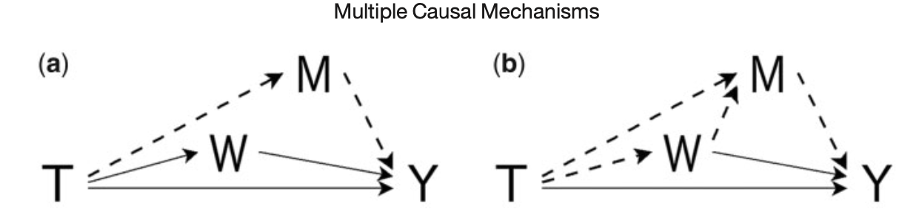
\includegraphics[width=\linewidth]{multiple_mechanisms}
	\end{figure}
	
	Formulate the framework for multiple mechanisms in terms of linear regression models, but there is more flexibility here. 
	\\~\\
	First, look at the Robins (2003) assumptions where:
	\begin{itemize}
		\item Treatment is exogenous given pretreatment covariates
		\item Mediator $M$ is exogenous given pre and post treatment covariates. 
		\item There is no interaction between treatment and mediator (i.e. the causal effect of the mediator on the outcome does not depend on treatment status).
	\end{itemize}
	~\\
	However, the assumption of no treatment-mediator interaction is often too strong. For example, in framing experiments the effect of an issue on opinions may depend on initial framing. We can thus relax the key identification assumption by developing sensitivity analysis. The key contribution here is thus sensitivity analysis to posttreatment confounders. 
	\\~\\
	A limitation of the approach is that it still hinges on an untestable assumption of no unmeasured confounder for the mediator. Suggest an experimental approach to deal with this, but that won't be relevant for observational studies. 
	\\~\\
	\textbf{Three motivating examples.} All to do with framing effects - can the framing of issues in mass media and elite communication affect citizens' political opinion and behaviour? In all cases there are multiple causal mechanisms that are independent of one another. 
	\begin{enumerate}
		\item Campaign Finance Reform Experiment: importance mechanism or content mechanism. 
		\item Social Welfare Reform Experiment: importance and content of the issue.
		\item Immigration Experiment: perceived harm mechanism or anxiety mechanism
	\end{enumerate}
	~\\
	In general mediation analysis usually involves fitting two linear regressions separately:
	$$
	M_i = \alpha_2 + \beta_2 T_i + \zeta_2 X_i + \epsilon_{i2}
	$$
	$$
	Y_i = \alpha_3 + \beta_3 T_i + \gamma M_i +  \zeta_3 X_i + \epsilon_{i3}
	$$
	where $X_i$ represents pretreatment confounders. After fitting the two models the ACME is $\beta_2 \gamma$ and $\beta_3 $ is the ADE. Following Imai, Keele and Yamamoto (2010) this can be justified under sequential ignorability. Sequential ignorability requires that there is no posttreatment confounding between the mediator and the outcome. In my case it means that there is no confounding between trading volume and volatility. 
	\\~\\
	Sequential ignorability (part 2) can fail for two reasons:
	\begin{enumerate}
		\item Unobserved pretreatment confounding
		\item Any posttreatment confounding
	\end{enumerate}
	So even if the mediator is exogenous after conditioning on a vector of posttreatment confounders ($W_i$) as well as $T_i$ and $X_i$ then sequential ignorability is violated and we can't identify the average mediation effect. Furthermore, the sensitivity analysis addresses the problem of potential unobserved pretreatment confounding, but it does not allow for the possibility of posttreatment confounding. 
	\\~\\
	Multiple mechanisms are by definition causally affected by the treatment and influence the outcome. If alternative mediators affect the mediator of interest, then it is easy to see that this violates sequential ignorability. 
	\\~\\
	We thus have two types of causal mediation effects - with respect to $M$ and $W$. 
	\\~\\
	Generalise the sequential ignorability assumption with multiple causally independent mediators. There are now three parts to the sequential ignorability assumption. 
	\begin{enumerate}
		\item The outcome and mediators are independent of treatment, conditional on pretreatment covariates 
		$$
		Y_i(t,m,w), M_i(t'), W_i(t'') \indep T_i | X_i = x
		$$
		\item The outcome and the alternative mediator are independent of the primary mediator, conditional on treatment and pretreatment covariates
		$$
		Y_i(t', m, W_i(t')) \indep M_i | T_i =t, X_i = x
		$$
		\item The outcome and primary mediator are independent of the alternative mediator, given the treatment and pretreatment covariates
		$$
		Y_i(t', m, M_i(t')) \indep W_i | T_i =t, X_i = x
		$$
	\end{enumerate}
	The standard analysis of multiple mediators in many social science applications relies implicitly on the is strong sequential ignorability assumption. 
	
	
	\subsection{Multiple Causal Mechanisms}
	
	Introduce potential values of $W$, where $W_i$ is a posttreatment variable and so possibly affected by the treatment. If there is no causal relationship between $M_i$ and $W_i$, then everything is fine. 
	\\~\\
	Here focus on cases where other mediators $W$ confound the relationship between $M$ and $Y$, so $M$ is exogenous conditional of $X$, $T$ and $W$.  $M$ is causally affected by a set of alternative mediators $W$. 
	\\~\\
	The mediated effect $\delta_i(t)$ is the causal effect of the treatment that transmits through the mediator of interest $M$. 
	\\~\\
	\textbf{Sequential Ignorability with Multiple Causally Dependent Mediators}.
	Assumption has three parts:
	\begin{enumerate}
		\item The outcome and both mediators are random wrt treatment, conditional on $X$. 
		$$
		Y_i(t,m,w), M_i(t,w), W_i(t) \indep T_i | X_i = x
		$$
		\item The outcome and the primary mediator are independent of the alternative mediator, conditional on treatment and $X$
		$$
		Y_i(t,m,w), M_i(t,w) \indep W_i(t) | T_i =t, X_i = x
		$$
		\item The outcome is independent of the primary mediator, conditional on alternate mediator, treatment and $X$
		$$
		Y_i(t,m,w) \indep M_i(t,w) | W_i(t) =w, T_i =t, X_i = x
		$$
	\end{enumerate}
	So this assumes that there may be a causal effect of $W$ through $M$, but not of $M$ through $W$. 
	\\~\\
	But, as shown by Robins (2003) we need an additional assumption of no treatment-mediator interaction for the ACME to be identified. 
	$$
	Y_i(1, m, W_i(1)) - Y_i(0,m,W_i(0)) = Y_i(1, m', W_i(1)) - Y_i(0,m',W_i(0))
	$$
	for any $m$, $m'$. SO I think this is saying that the effect of $W$ on $Y$ must be independent of $M$. 
	\\~\\
	It looks like they're arguing you can relax the no interaction assumption and just rely on the three part sequential ignorability assumption. 
	$$
	M_i(t,w) = \alpha_2 + \beta_{2i} t + \zeta_{2,i}w + \mu_{2i} t  w + \lambda_{2i} x + \epsilon_{2i}
	$$
	$$
	Y_i(t,m,w) = \alpha_3 + \beta_{3i} t + \gamma_i m + \kappa_i t m + \zeta_{3,i} w + \mu_{3i} t  w + \lambda_{3i} x + \epsilon_{3i}
	$$
	This reflects the situation in Figure (b). Specifically, $M$ depends on a set of alternative mediators $W$ which is possibly affected bu the treatment as well as the treatment $T$. 
	
	
	
	
	
	 
	
	
	

	
	
	
	
	
	
	
	
	
	
	
	
	
	
	
	
	\section{Causal Mediation for media coverage effect}
	
	In this case $Y_i$ is the intraday high-low spread, $T_i$ is media coverage and $M_i$ is trading volume. $X_i$ are the pre-treatment confounders including past price movements and implied volatility, fixed effects and other firm or period level information. 
	\\~\\
	The sequential ignorability assumption then that (i) media coverage is random once we adjust for differences in past performance, implied volatility and firm/time specific factors; (ii) trading volume is random once taking into account differences in media coverage, past performance, implied volatility and firm/time specific factors. 
	\\~\\
	For sequential ignorability to imply identification of the ACME, we can only condition on pre-treatment variables. We cannot condition on pre-mediator confounders if they are affected by the treatment. So, for example, we cannot condition Volume on intra-day return if return is also affected by the media coverage.
	\\~\\
	The sensitivity analysis in this context would involve a confounder that is correlated with the volatility and volume errors. So for example if there is some anticipated information event that drives both volatility and volume then the errors would be positively correlated. So we can test how strong this correlation needs to be for the effect to disappear. 
	\\~\\
	If there are multiple causal relationships then sequential ignorability is satisfied only if the two mediators are causally unrelated. In our case this would mean that return magnitude and Volume are causally unrelated. 
	\\~\\
	Including the intra day return thus violates the sequential ignorability assumption, but we can include it as a lower bound on the results. 
	
	
	\begin{table}[!htbp] \centering 
		\caption{} 
		\label{} 
		\footnotesize
		\begin{tabular}{@{\extracolsep{-3pt}} ccccccccccc} 
			\\[-1.8ex]\hline 
			\hline \\[-1.8ex] 
			& AGEP & health & wage & wage\_zeros & wage\_imp & AGEP.1 & health.1 & wage.1 & wage\_zeros.1 & wage\_imp.1 \\ 
			\hline \\[-1.8ex] 
			AGEP & 1 &  &  &  &  & 1 &  &  &  &  \\ 
			health & -0.31 & 1 &  &  &  & -0.293 & 1 &  &  &  \\ 
			wage & 0.084 & 0.149 & 1 &  &  & 0.113 & 0.132 & 1 &  &  \\ 
			wage\_zeros & -0.118 & 0.213 & 1 & 1 &  & -0.09 & 0.201 & 1 & 1 &  \\ 
			wage\_imp & -0.053 & 0.215 & 1 & 0.938 & 1 & -0.017 & 0.214 & 1 & 0.918 & 1 \\ 
			\hline \\[-1.8ex] 
		\end{tabular} 
	\end{table}
	\begin{table}[!htbp] \centering 
		\caption{} 
		\label{} 
		\footnotesize
		\begin{tabular}{@{\extracolsep{-3pt}} ccccccccccc} 
			\\[-1.8ex]\hline 
			\hline \\[-1.8ex] 
			& AGEP & health & wage & wage\_zeros & wage\_imp & AGEP.1 & health.1 & wage.1 & wage\_zeros.1 & wage\_imp.1 \\ 
			\hline \\[-1.8ex] 
			AGEP & 1 &  &  &  &  & 1 &  &  &  &  \\ 
			health & -0.287 & 1 &  &  &  & -0.27 & 1 &  &  &  \\ 
			wage & 0.136 & 0.12 & 1 &  &  & 0.115 & 0.117 & 1 &  &  \\ 
			wage\_zeros & -0.088 & 0.202 & 1 & 1 &  & -0.11 & 0.195 & 1 & 1 &  \\ 
			wage\_imp & 0.009 & 0.21 & 1 & 0.911 & 1 & -0.004 & 0.204 & 1 & 0.913 & 1 \\ 
			\hline \\[-1.8ex] 
		\end{tabular} 
	\end{table} 
	~\\
	\textbf{On anticipating high volatility.} It is to some extent an open question whether the media \textit{causes} volatility or whether it is very good at anticipating it. However, by controlling for implied volatility, we do get an indication that if the media is anticipating volatility it is more adept at doing so than financial markets are.    
	\
	
\end{document}
